\documentclass{beamer}
\usetheme{Copenhagen}
\usecolortheme{whale}
\usefonttheme[onlymath]{serif}

\usepackage{setspace}
\usepackage{xcolor}
\usepackage{graphicx}
\usepackage{multimedia}
\usepackage{fontawesome}
\usepackage[most]{tcolorbox}
\usepackage{empheq}
\usepackage{fancybox}

\title{Answering questions by combining data sources}
\author[Zivich]{Paul Zivich \\~\\ Institute of Global Health and Infectious Diseases \\ University of North Carolina at Chapel Hill}

\setbeamercovered{transparent}
\setbeamertemplate{navigation symbols}{}  % gets rid of the dumb navigation symbols
\setbeamertemplate{page number in head/foot}{\insertframenumber}  % adds slide #
\setbeamertemplate{headline}{}

\AtBeginSection[]{
	\begin{frame}
		\vfill
		\centering
		\begin{beamercolorbox}[sep=8pt,center,shadow=true,rounded=true]{title}
			\usebeamerfont{title}\insertsectionhead\par%
		\end{beamercolorbox}
		\vfill
	\end{frame}
}

\begin{document}

\begin{frame}
    \maketitle
\end{frame}

\begin{frame}{Acknowledgements}
	Supported by NIH T32-AI007001\\~\\~\\
	
	\centering
	\faEnvelope \quad pzivich@unc.edu \qquad
	\faGithub \quad pzivich\\
\end{frame}

\begin{frame}{Why Multiple Data Sources?}
	A single data source may be unable to adequately address pressing public health questions 
	\begin{itemize}
		\item Measurement error, convenience sample
	\end{itemize}~\\
	To address these biases
	\begin{itemize}
		\item Integrate information across multiple sources of information
	\end{itemize}
\end{frame}

\begin{frame}{An Analogy}
	\centering
	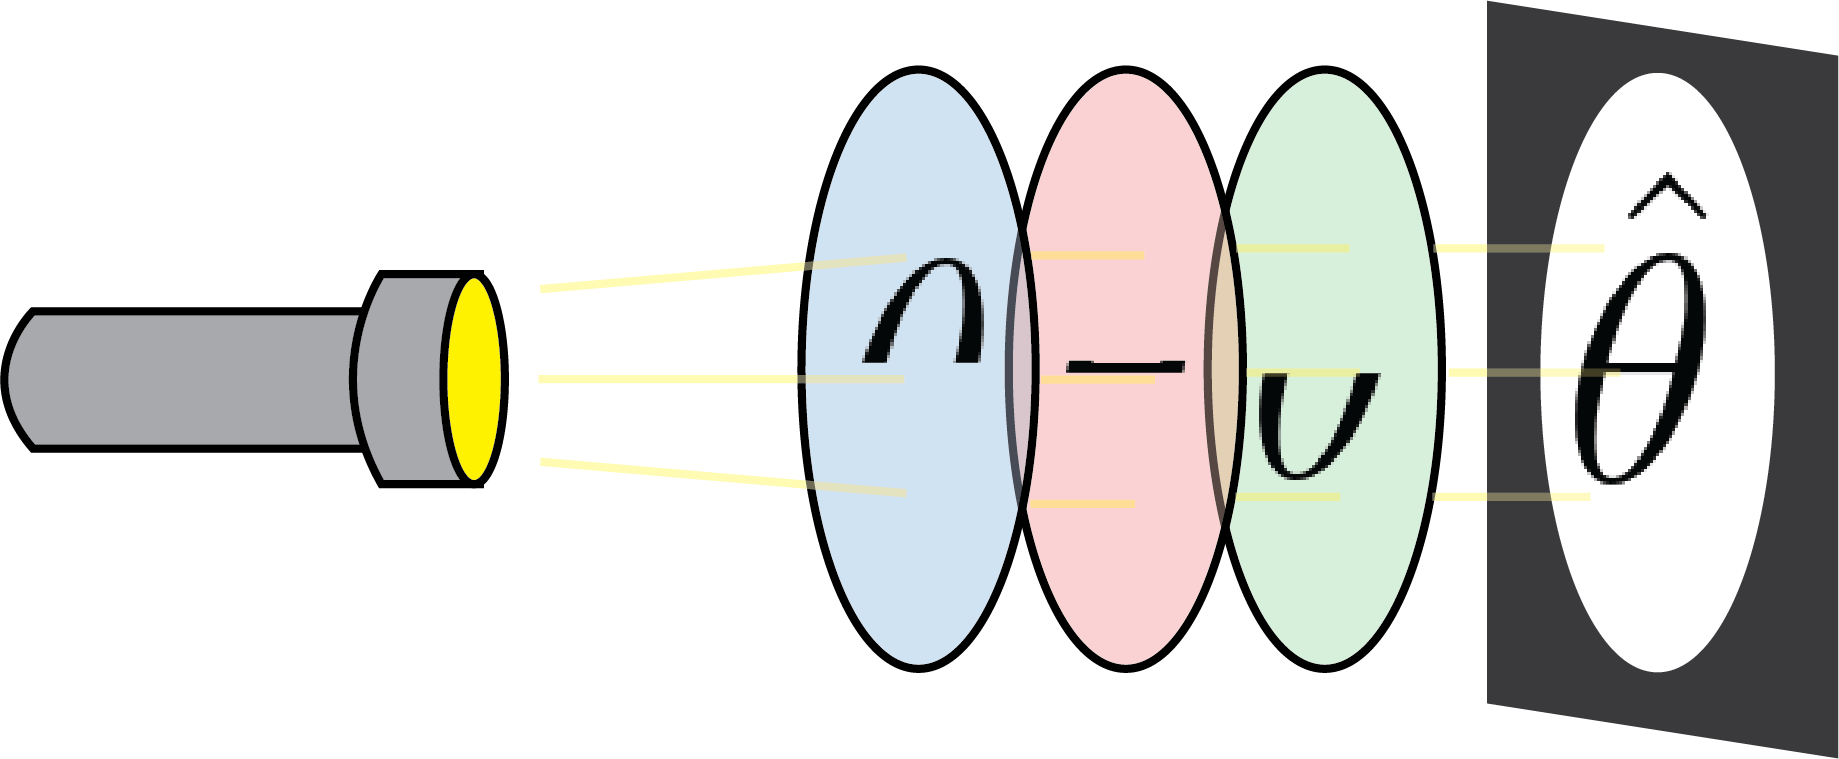
\includegraphics[width=0.9\linewidth]{fusion_analogy1.png}
\end{frame}

\begin{frame}{An Analogy}
	\centering
	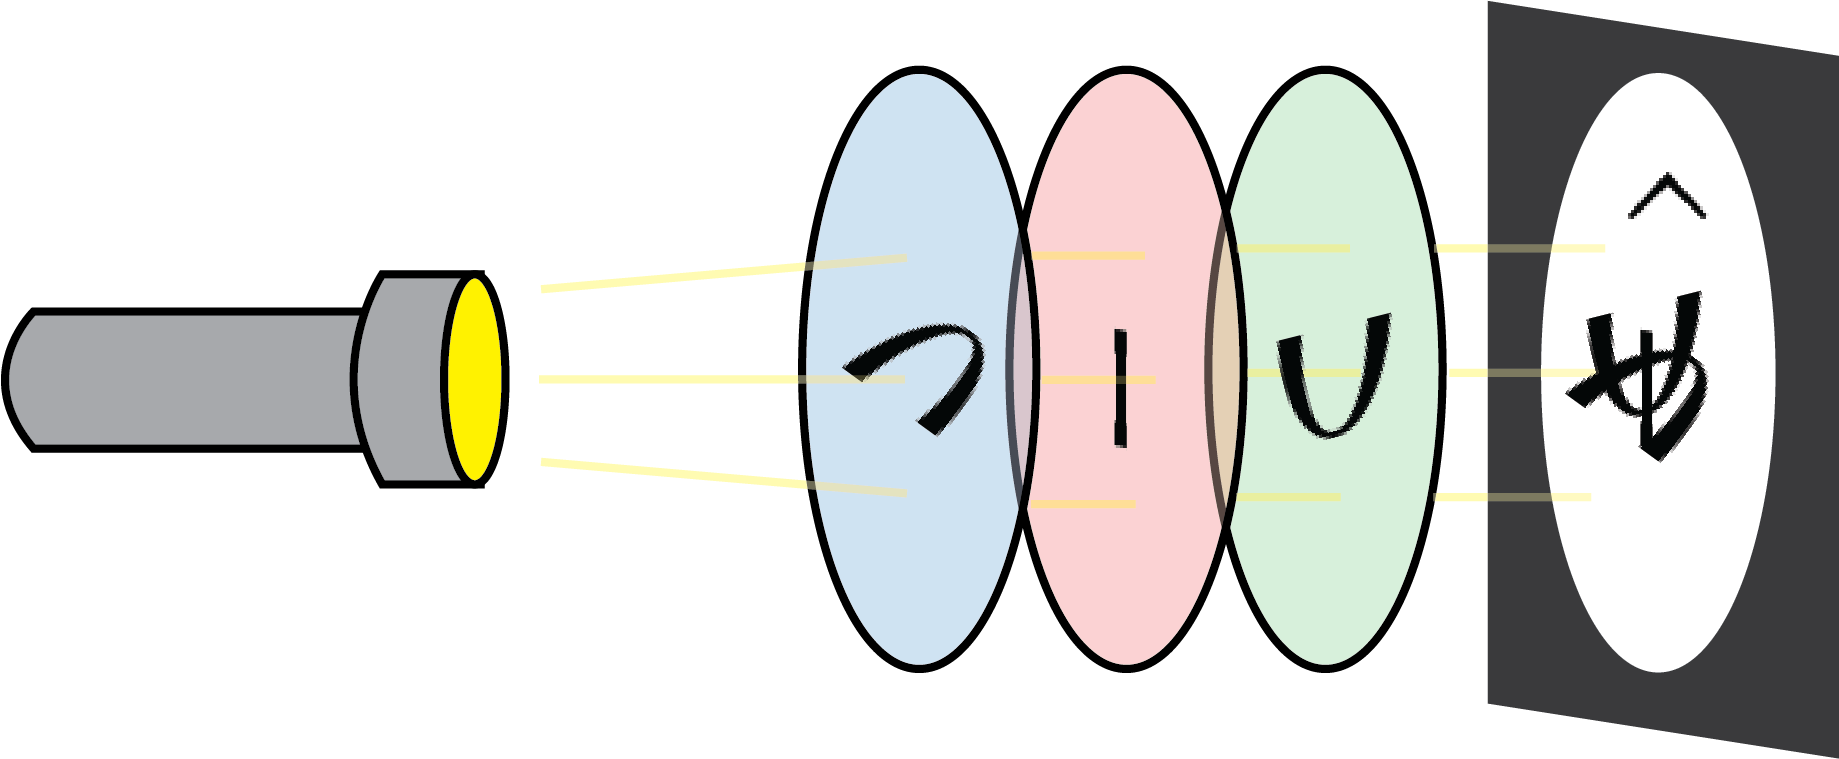
\includegraphics[width=0.9\linewidth]{fusion_analogy2.png}
\end{frame}

\begin{frame}{Historical Perspective}
	Use of multiple data sources has a long history
	\begin{itemize}
		\item Case-control studies\footnote[frame]{Lane-Claypon (1926) Reports on Public Health and Medical Subjects 32}
		\item Validation studies for measurement error\footnote[frame]{Rogan \& Gladen (1978) \textit{Am J Epidemiol}}
		\item Meta-analysis\footnote[frame]{ Glass (1978) \textit{Educ Researcher}}
		\item Two-stage studies\footnote[frame]{Zhao \& Lipsitz (1992) \textit{Stats in Med}}
		\item Mathematical modeling\footnote[frame]{Bernoulli (1776) \textit{Mem Math Phy Acad Roy Sci Paris}}
	\end{itemize}
\end{frame}

\begin{frame}{Modern Perspective}
	Recently, approaches have been sharpened
	\begin{itemize}
		\item Lens of causal inference
		\item Generally proceeded under the generalizability\footnote[frame]{Cole \& Stuart (2010) \textit{Am J Epidemiol}} and transportability\footnote[frame]{Bareinboim \& Pearl (2016). \textit{PNAS}} framework
		\begin{itemize}
			\item Acknowledgment of conditions to combine data sources
			\item Alignment in flashlight analogy
		\end{itemize}
	\end{itemize}
\end{frame}

\begin{frame}{Purpose of the Session}
	Learn about recent developments in the integration of information across sources from a variety of perspectives
	\begin{itemize}
		\item Hear from different perspectives
		\item Lead to future improvements
	\end{itemize}
\end{frame}

\begin{frame}{Speakers}
	Stephen Cole
	\begin{itemize}
		\item Combining sources of information using a data fusion perspective
	\end{itemize}
	Issa Dahabreh
	\begin{itemize}
		\item Combining information from multiple sources to learn about a target popoulation: meta-analysis and beyond
	\end{itemize}
	Eric Lofgren
	\begin{itemize}
		\item `Just Bring Me Everything' Data Fusion in Mathematical Model Fitting and Parameterization
	\end{itemize}
	Leon Di Stefano
	\begin{itemize}
		\item Careful hierarchical Bayesian modelling for pooling information across trials
	\end{itemize}
	Summary \& Panel Discussion
\end{frame}

\end{document}
